%% Electro-optic study of AlGaAs coated mirrors

As mentioned in Section (1?) one of the many LIGO fundamental noise sources is coating thermal noise from the $\mathrm{SiO}_2-\mathrm{TaO}_5$ ALIGO coating. As ALIGO approaches its designed sensitivity various coating solutions are currently proposed to mitigate thermal noise coupling into the detector output.
With the potential to reduce noise by a factor of 5, AlGaAs shows much promise with next generation detectors, though with different material properties of this crystalline coating introduces new coating noise couplings. A notable source of noise is the linear electro-optic property of the crystal (dn/dE), also known as the Pockels effect.  Characterizing currently proposed AlGaAs coated "witness" samples thorough extensive analysis and experimental data of the aforementioned properties is essential for the use of AlGaAs in gravitational wave interferometers. The following section dedicated to the discussion of said properties starting with the fundamentals on the Pockels effect, the coupling mechanism and estimates of coupling.


\subsection{The Pockels Effect}
This property of anisotropic crystalline media (ACM) explains the depdendence of the index of refraction of a material with a relatively slowly varying (with respect to the EM radiation) Electric field . This property of ACM is what allows electro-optic modulators to operate as light phase modulators\cite{yariv} \cite{nye}. \textcolor{red}{More to be discussed: How the modulation of the phase of the carrier field is dependent on the orientation of its wave vector with respect to the crystal structure, the modulating electric field direction and strength, (other items to discuss in terms of introducing the effect)  }


\section{Phase modulation of light propogating through stratified anisotropic crystalline media}

\subsection{Coating parameters}
\textcolor{red}{Info from Steve:
$\lambda$ / 4 stack.  It is 36 layers of GaAs interspersed with 35 layers of AlGaAs.   GaAs forms the top and bottom layer to protect the AlGaAs from absorbing oxygen from the air.
High Index:  GaAs, n=3.480, layer thickness is 76.43 nm
Low Index:  $ \mathrm{Al}_{0.92} \mathrm{Ga}_{0.08} \mathrm{As} $, n=2.977, layer thickness is 89.35 nm}

\subsection{Fejer and Bonilla approach}
Fejer and Bonilla take an analytical approximation approach when finding the impact of the Electric field to the change in phase of the light through a crystalline anisotropic media.

\subsection{Ballmer approach}



\section{Projected DARM coupling}

\section{Experiment}

\subsection{Design}
Short in-air cavity with a PDH lock.

\begin{figure}[H]
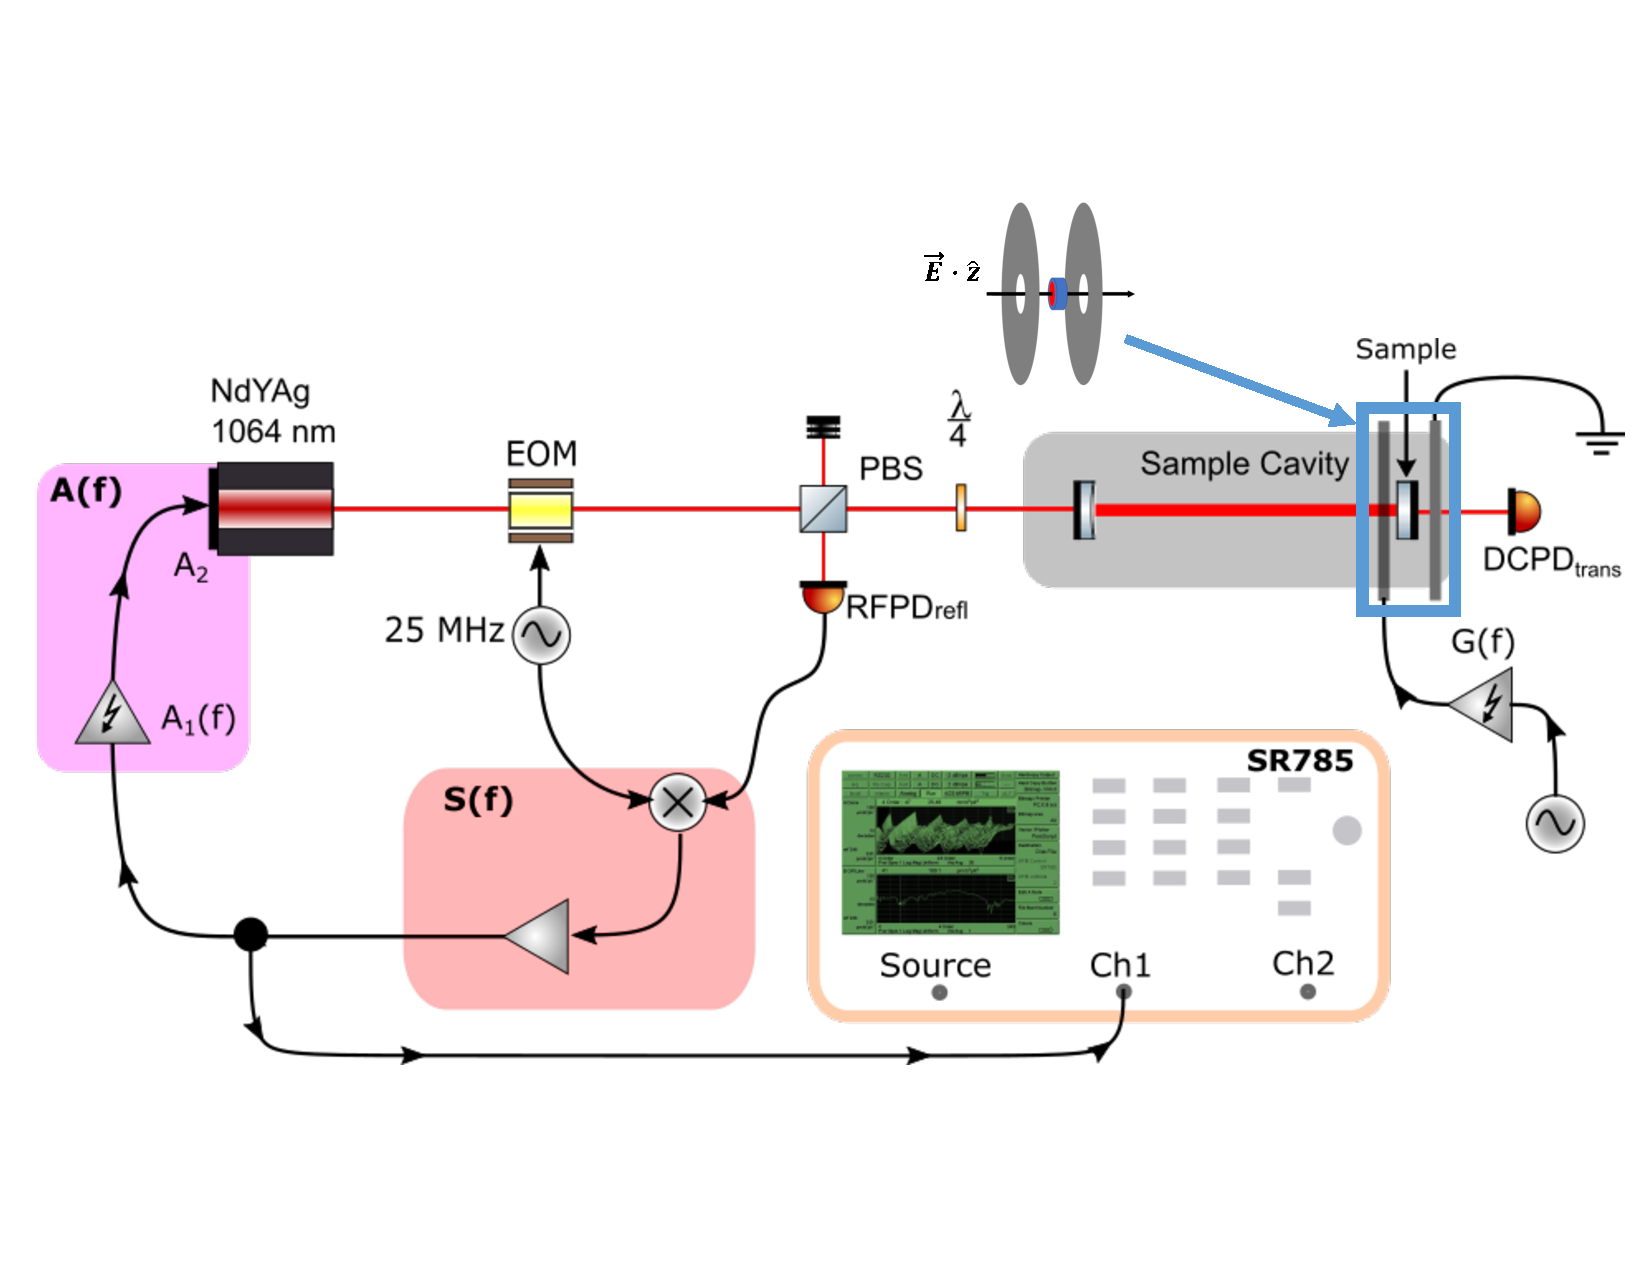
\includegraphics[width=\textwidth]{ALGAAS/algaas_pockels_effect_measurement_schematic}
\caption{Experiment schematic. Needs to be updated with the Agilent 4395A analyzer.}
\label{fig:poisson_output}
\end{figure}

Maximizing the electric field normal to the sample coating ($|E_z|$) within the coating. Given a chosen aperture size (established by choosing the an aperture size that is 5 times larger than the beam size). An optical mount for the sample made with MACOR, along with glass bearnings and a McMaster-Carr 8-32, 1/2" ceramic screw were used to There are two relevant configurations of this experiment: 1) an all-in-one MACOR assembly where the electrodes are mechanically coupled to the optical mount, and 2) larger mechanically decoupled electrode plates.



\subsection{$|E_z|$ strength}
\begin{figure}[H]
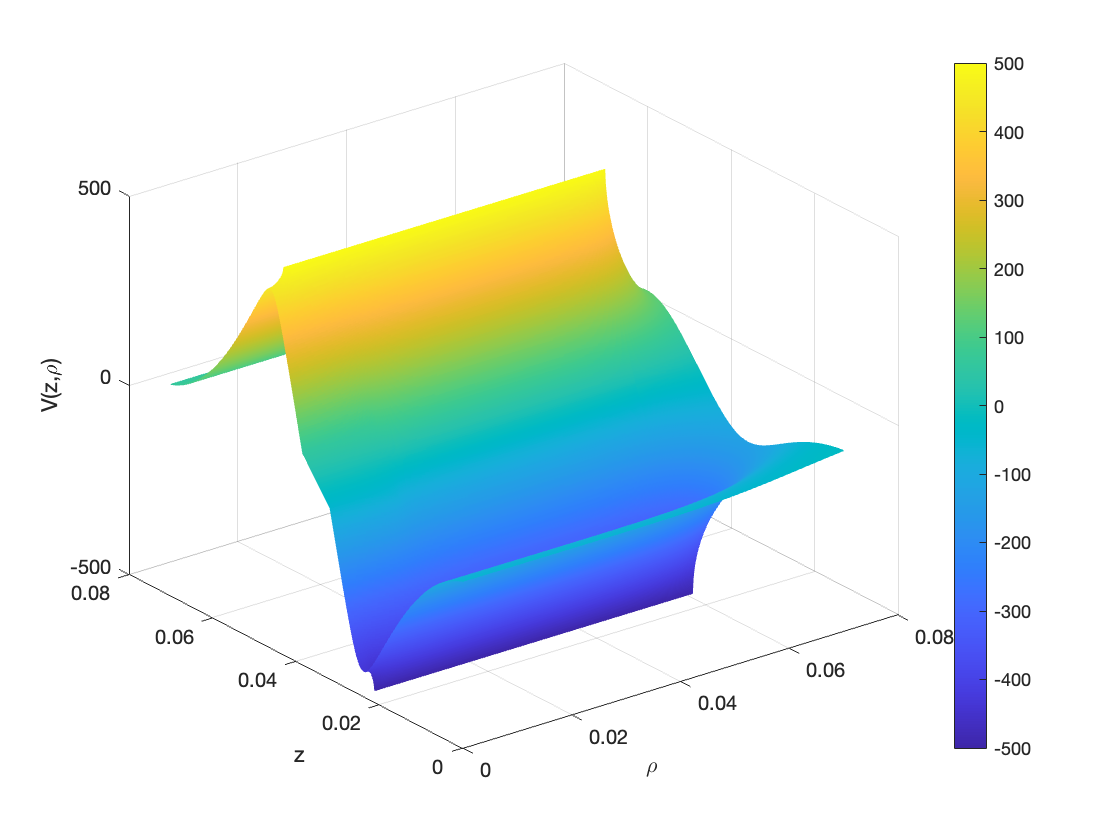
\includegraphics[width=\textwidth]{ALGAAS/13-Sep-2021_potential_map}
\caption{Poisson calculator output potential map ($V(z,\rho)$)}
\label{fig:poisson_calc_output}
\end{figure}

\begin{figure}[H]
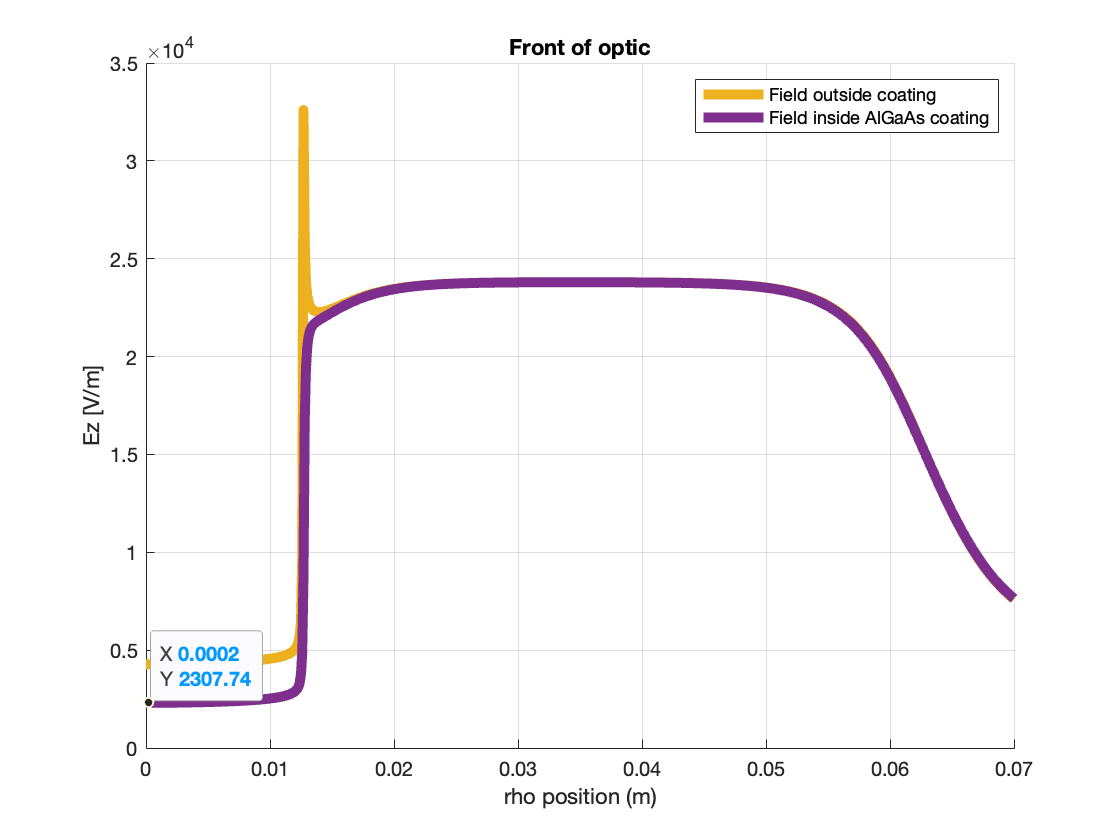
\includegraphics[width=\textwidth]{ALGAAS/13-Sep-2021_e_field_inside_outside_normal}
\caption{$|E_z|$ screened by coating and $|E_z|$ immediately outside AlGaAs coating}
\label{fig:Ez}
\end{figure}

TREK 10/10B-HS HVA frequency depdendent measurement. Using Poisson calculator to estimate field strength within coating

\subsection{Calibration}

$V_\mathrm{FSSOUT} \rightarrow m_\mathrm{rms}/\sqrt{\mathrm{Hz}}$

$$\Delta L = \mathrm{source}*\alpha(f) A(f)*\frac{1+OLG(f)}{OLG(f)}*\frac{L_\mathrm{cav}}{f_\mathrm{laser}}$$

\subsection{Noise Floor}

\subsection{Drive coupling}

\begin{figure}[H]
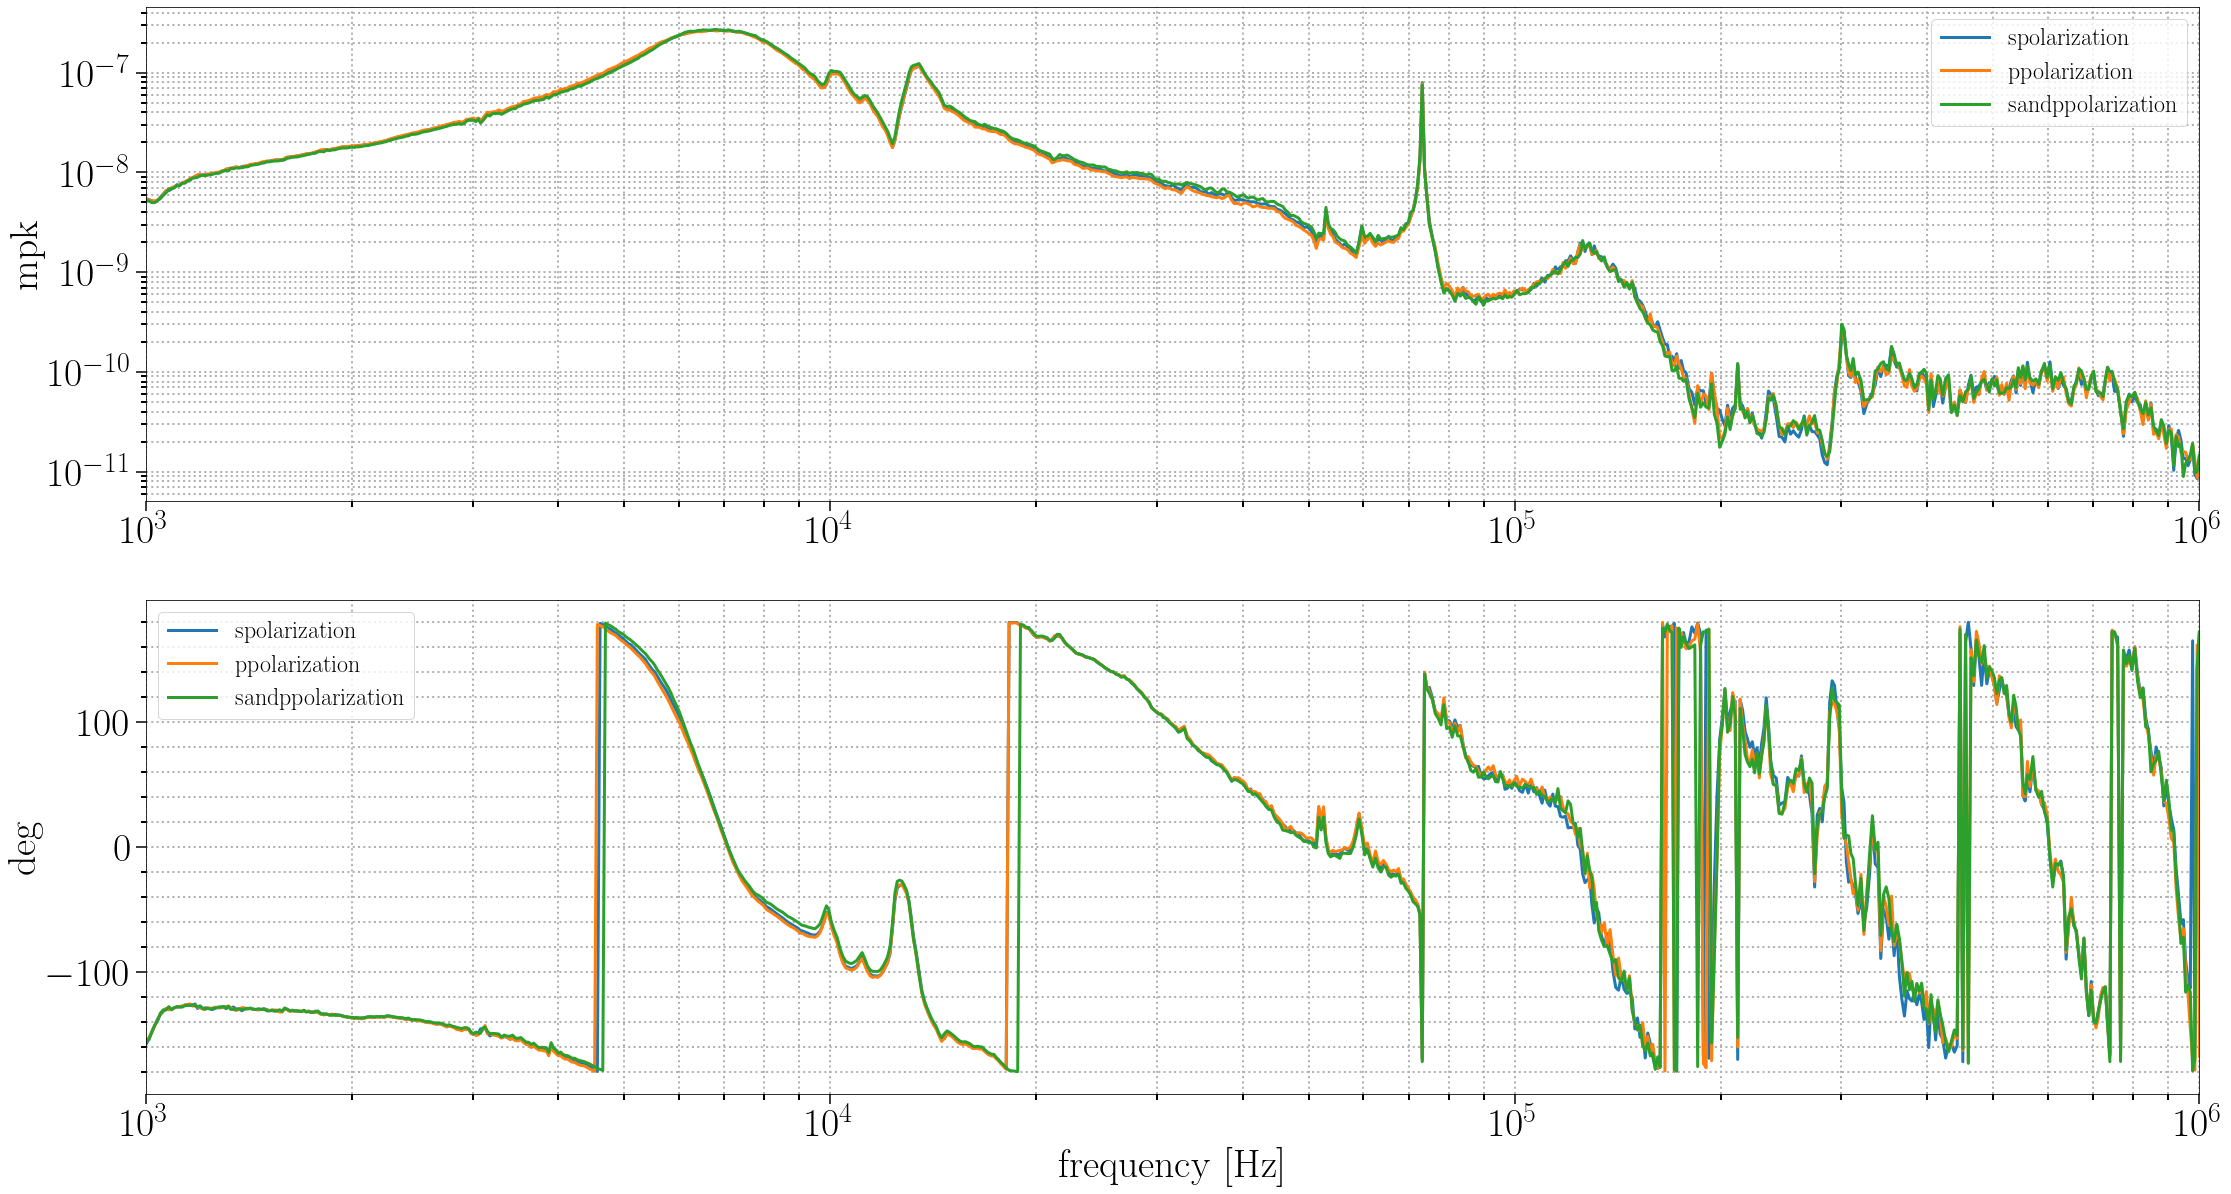
\includegraphics[width=\textwidth]{ALGAAS/calibrated_polarization_test}
\caption{Figure that will include the displacement noise floor, (pockels estimate)*(poisson calculator estimate)*(HVA drive frequency dependence), and the drive coupled measurement \textcolor{red}{figure size needs to be increased}}
\label{fig:measurement_sum}
\end{figure}

\subsubsection{Mechanical modes}
Sample and mount mechanical mode excitations. Seen with both AlGaAs and a HR coating from an AtFilm (IBS coating)
\\
\textbf{Vibration of plates (Leissa)}
Computing frequency and order of magnitude
\\
\textbf{Steve's COMSOL model}
